\documentclass[12pt, a4paper]{article}

% Preamble
\usepackage{xeCJK}
\usepackage[utf8]{inputenc}
\usepackage[english]{babel}
\usepackage[margin=1in]{geometry}
\usepackage[parfill]{parskip}
\usepackage{listings}
\usepackage{graphics}
\usepackage{graphicx}
\usepackage{nasm/lang}
\usepackage{nasm/style}
\usepackage{c/style}
\usepackage{go/lang}
\usepackage{go/style}
\usepackage{reil/lang}
\usepackage{llvm/lang}
\usepackage{diff/lang}
\usepackage{diff/style}
\usepackage{dot/lang}
\usepackage{dot/style}
\usepackage{float}
\usepackage[colorlinks,linkcolor=blue]{hyperref}
\usepackage{mips}

\usepackage{listings}
%\usepackage{color}

% Document

\usepackage{etoolbox}
\makeatletter
\def\@xobeysp{\hspace{0pt}\mbox{ }\hspace{0pt}}
\appto\verbatim@font{\hyphenchar\font`-\relax}
\apptocmd\@sverb{\hspace*{0pt}}{}{}
\makeatother


\definecolor{dkgreen}{rgb}{0,0.6,0}
\definecolor{gray}{rgb}{0.5,0.5,0.5}
\definecolor{mauve}{rgb}{0.58,0,0.82}
\definecolor{vgreen}{RGB}{104,180,104}
\definecolor{vblue}{RGB}{49,49,255}
\definecolor{vorange}{RGB}{255,143,102}
\lstdefinestyle{verilog-style}
{
	language=Verilog,
	basicstyle=\small\ttfamily,
	breaklines=true,
	showstringspaces=false,
	columns=flexible,
	keywordstyle=\color{vblue},
	identifierstyle=\color{black},
	commentstyle=\color{vgreen},
	numbers=left,
	numberstyle=\tiny\color{black},
	numbersep=7pt,
	tabsize=4,
	literate=*{:}{{\textcolor{black}{:}}}1
}

\lstdefinestyle{MIPS}
{
	language=[mips]Assembler,       % the language of the code
	basicstyle=\footnotesize,       % the size of the fonts that are used for the code
	numbers=left,                   % where to put the line-numbers
	numberstyle=\tiny\color{gray},  % the style that is used for the line-numbers
	stepnumber=1,                   % the step between two line-numbers. If it's 1, each line 
	% will be numbered
	numbersep=5pt,                  % how far the line-numbers are from the code
	backgroundcolor=\color{white},  % choose the background color. You must add \usepackage{color}
	showspaces=false,               % show spaces adding particular underscores
	showstringspaces=false,         % underline spaces within strings
	showtabs=false,                 % show tabs within strings adding particular underscores
	frame=single,                   % adds a frame around the code
	rulecolor=\color{black},        % if not set, the frame-color may be changed on line-breaks within not-black text (e.g. commens (green here))
	tabsize=4,                      % sets default tabsize to 2 spaces
	captionpos=b,                   % sets the caption-position to bottom
	breaklines=true,                % sets automatic line breaking
	breakatwhitespace=false,        % sets if automatic breaks should only happen at whitespace
	title=\lstname,                 % show the filename of files included with \lstinputlisting;
	% also try caption instead of title
	keywordstyle=\color{blue},          % keyword style
	commentstyle=\color{dkgreen},       % comment style
	stringstyle=\color{mauve},         % string literal style
	escapeinside={\%*}{*)},            % if you want to add a comment within your code
	morekeywords={*,...}               % if you want to add more keywords to the set
}

\title{COD\_LAB5 多周期MIPS-CPU}
\author{黄业琦 PB17000144}
\date{May 7, 2019}
\begin{document}
\maketitle
\tableofcontents
\clearpage

\section{实验目的}
设计实现多周期MIPS-CPU,可执行如下指令:
\begin{itemize}
\item add, sub, and, or, xor, nor, slt
\item addi, andi, ori, xori, slti
\item lw, sw
\item beq, bne, j
\end{itemize}
数据通路和控制单元(状态图)参见后页,其中寄存器堆中R0内容恒定为0,存储器容量为256x32位。
\begin{figure}[H]
	\centering
	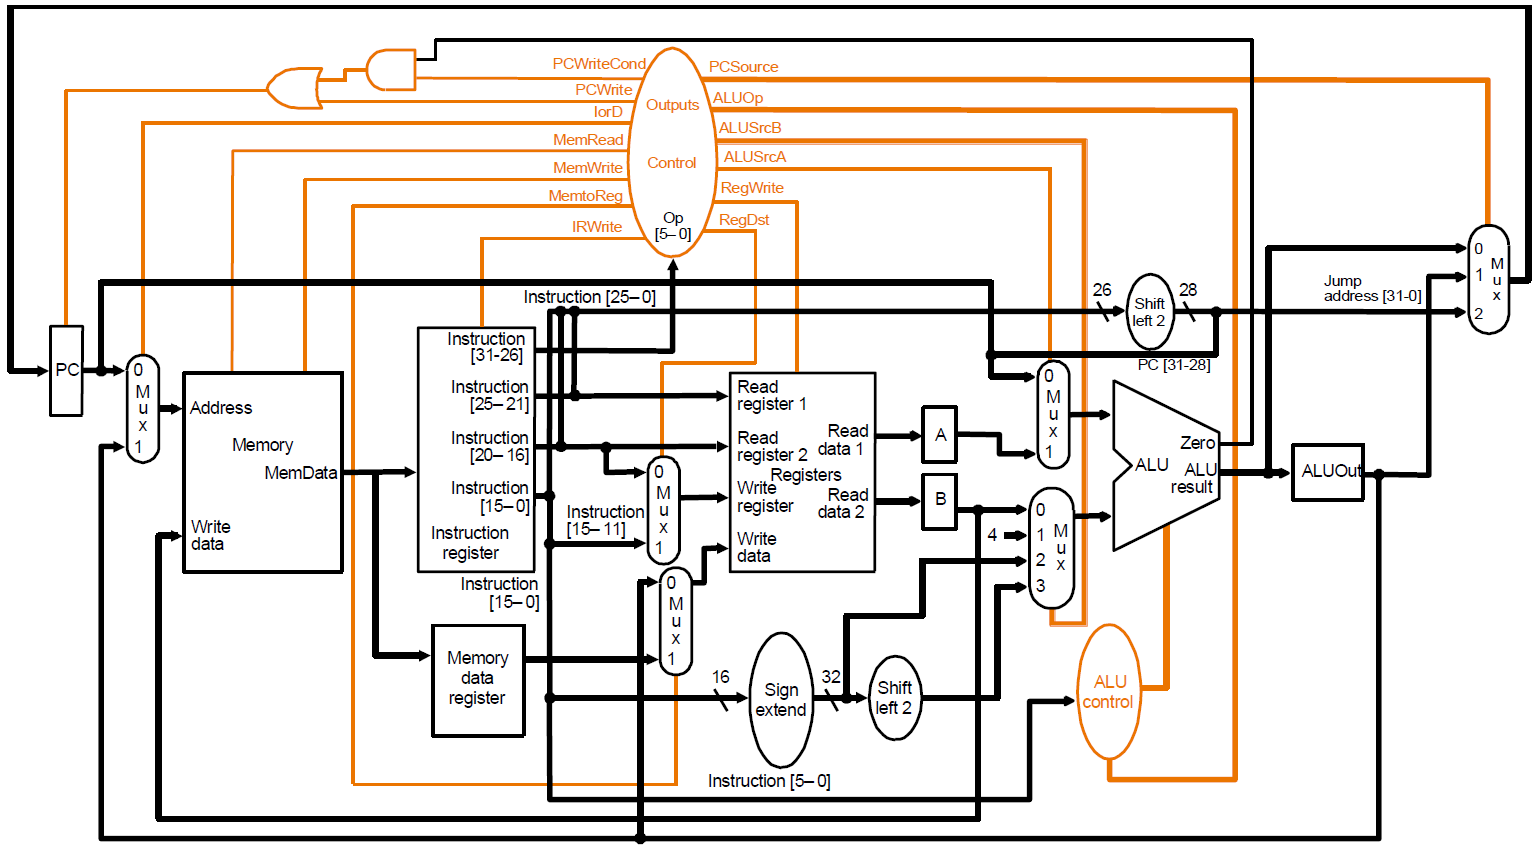
\includegraphics[width=1\linewidth]{pics/Picture1}
	\caption{Route1}
	\label{fig:picture1}
\end{figure}
DDU:Debug and Display Unit,调试和显示单元 \\
下载测试时,用于控制CPU运行方式和显示运行结果 \\
数据通路中寄存器堆和存储器均需要增加1个读端口,供DDU读取并显示其中内容 \\
\begin{figure}[H]
	\centering
	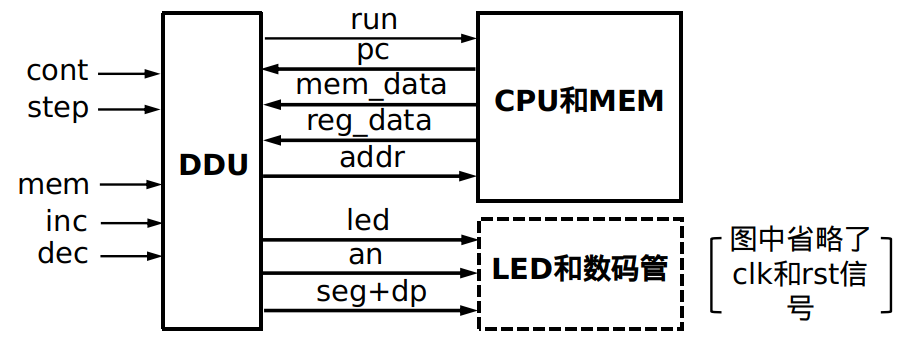
\includegraphics[width=1\linewidth]{pics/pc}
	\caption{DDU}
	\label{fig:pc}
\end{figure}
控制CPU运行方式:
\begin{itemize}
\item cont = 1:run = 1,控制CPU连续执行指令
\item cont = 0:每按动step一次,run输出维持一个时钟周期的脉冲,控制CPU执行一条指令
\end{itemize}
查看CPU运行状态:
\begin{itemize}
\item mem: 1,查看MEM;0,查看RF
\item inc/dec:增加或减小待查看RF/MEM的地址addr
\item reg\_data/mem\_data:从RF/MEM读取的数据
\item 8位数码管显示RF/MEM的一个32位数据
\item 16位LED指示RF/MEM的地址和PC的值
\end{itemize}

\section{实验环境}
Linux下编程调试和仿真,使用IVerilog,GtkWave系列工具。\\
Windows下用于生成比特流文件,使用Vivado 2018.2,Verilog HDL\\
所有下载均在Nexsy4-DDR实验板完成。\\
优秀的代码风格和规范的代码格式也很重要,本次实验借助Vscode的verilog-format插件进行整理代码的工作。

\section{逻辑设计}
代码逻辑结构参照我们的Figure1:Route1,但是我们需要做一点修改以方便编程实现。我们为了简化beq和bne,我们需要额外增加一个加法器,专门实现imm和pc的相加。
\begin{figure}[H]
	\centering
	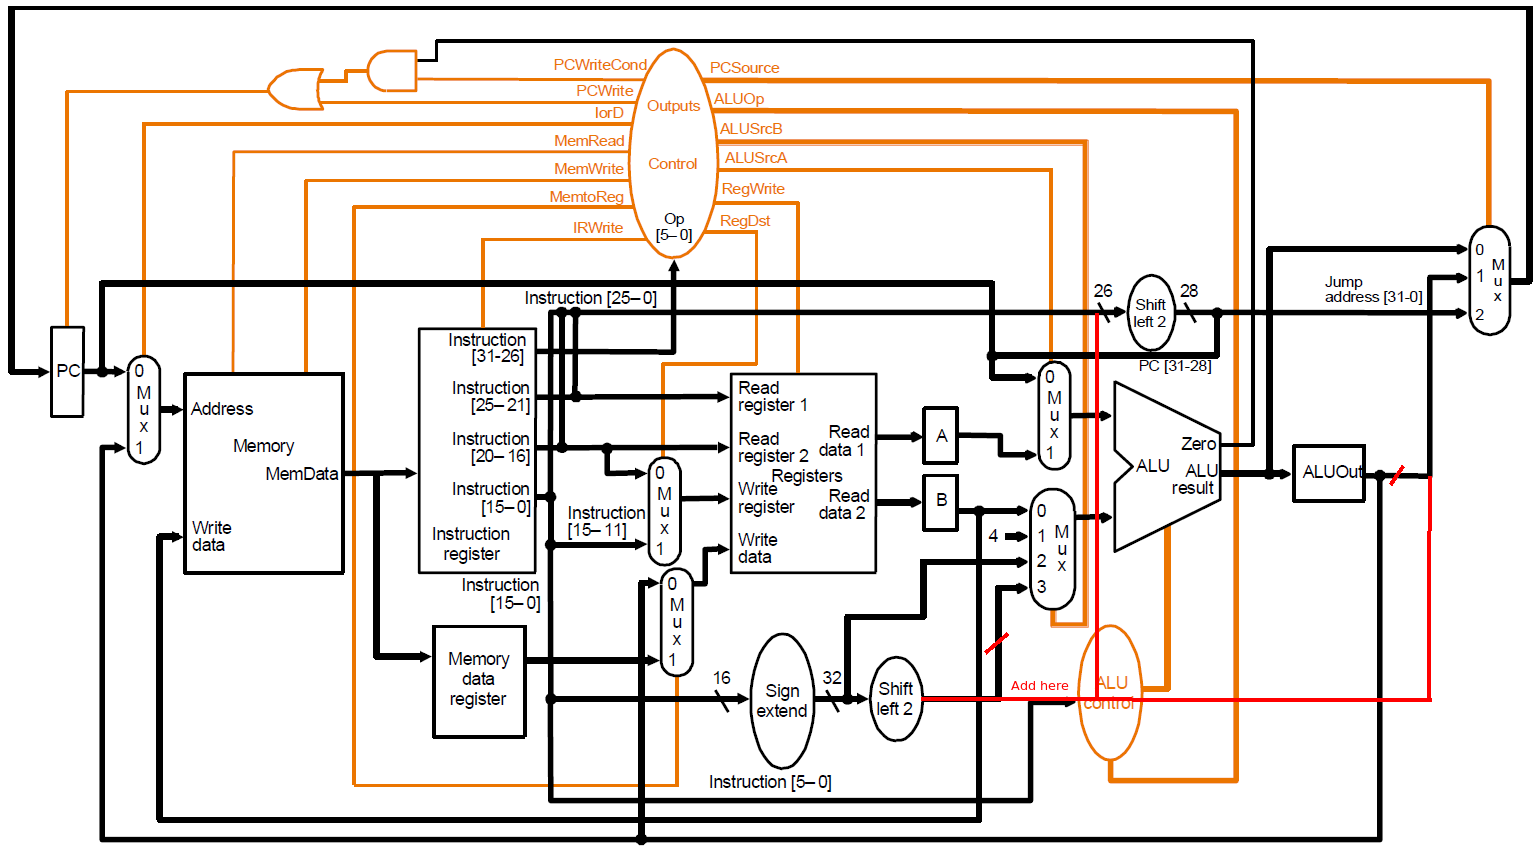
\includegraphics[width=1.0\linewidth]{pics/route}
	\caption{New Route}
	\label{fig:pic}
\end{figure}
关于逻辑结构,我们使用有限状态机进行描述。我们讲义给定的参考状态图是Figure:fsm,但是我们图中并没有我们关于I-type的算数运算的状态,为了弥补这一问题,我们对于一个状态进行了调整:fsm\_new。
\begin{figure}[H]
	\centering
	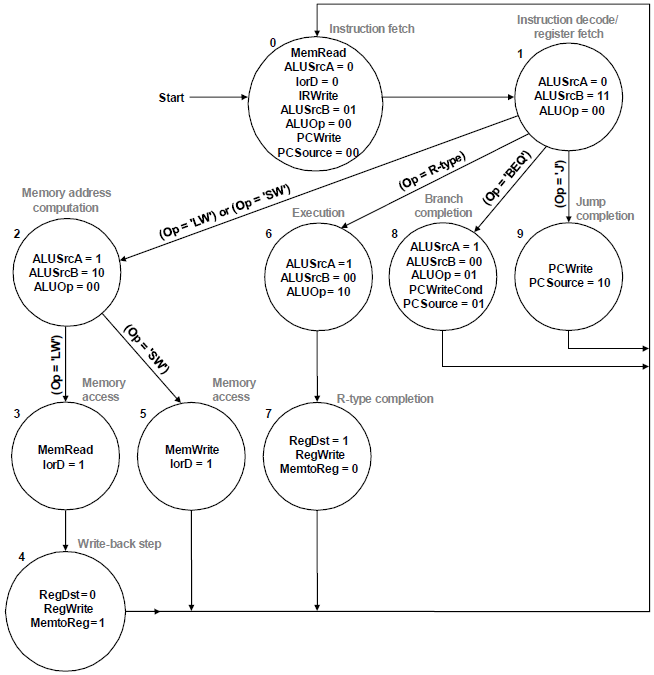
\includegraphics[width=1.0\linewidth]{pics/Picture2}
	\caption{FSM}
	\label{fig:fsm}
\end{figure}
\begin{figure}[H]
\centering
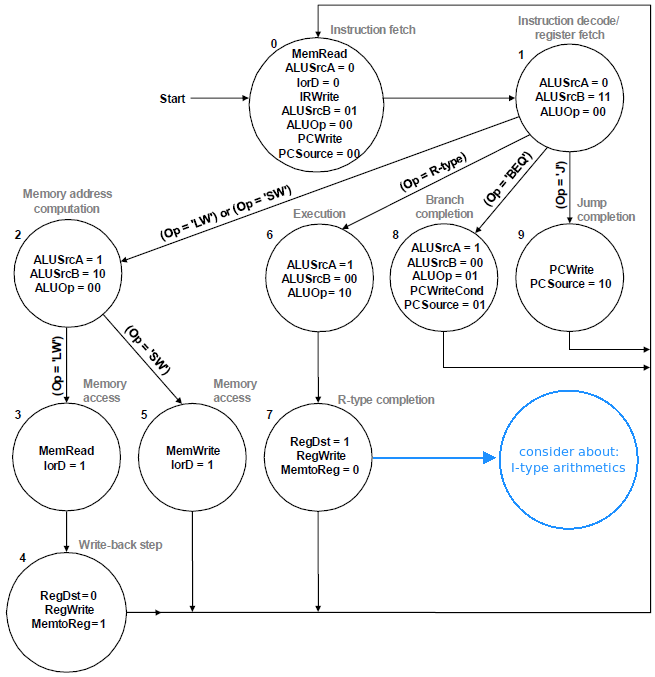
\includegraphics[width=1.0\linewidth]{pics/fsm}
\caption{FSM\_new}
\label{fig:fsm_new}
\end{figure}

这样我们就可以处理关于立即数计算的指令。\\
同时为了适应简化后的设计线路图,我们还做了以下改动:
\begin{enumerate}
\item 我们将aluop设作虚设,不做使用。
\item alusrcb只有一位就足以区分,关于pc的处理单独设立的新的加法器。
\item alusrca的值进行了小调整。
\item 关于bne和beq的设计。再alu中新添加了Compare equal的功能,这一设计个人认为十分巧妙在pc\_reg中有具体介绍这么做的原因。
\end{enumerate}
状态机的详细设计再define文件中有相应的描述。\\
状态设计如下,注释已经详细介绍了各个状态的具体功能。
\lstset{language = verilog, caption = State design}
\begin{lstlisting}
`define IF_STATE    4'b0000 // * if state
`define ID_STATE    4'b0001 // * id state
`define EXE1_STATE  4'b0010 // * exe for lw or sw
`define EXE2_STATE  4'b0011 // * exe for add/sub...(R&I type together)
`define EXE3_STATE  4'b0100 // * exe for branch (beq & bne)
`define EXE4_STATE  4'b0101 // * exe for j inst
`define MEM1_STATE  4'b0110 // * mem for lw - memread
`define MEM2_STATE  4'b0111 // * mem for sw - memwrite
`define WB1_STATE   4'b1000 // * write back for memory inst
`define WB2_STATE   4'b1001 // * write back for add/sub...
\end{lstlisting}

关于代码,采用模块化的设计,各模块及其功能如下(顺序为字典序):
\begin{itemize}
	\item IP核 clk\_wiz:  避免时钟周期过短。
	\item IP核 dist\_mem: 实现内存。
	\item alu: 实现运算器,纯组合逻辑。
	\item alu\_ctrl: 将指令的opcode和funt部分转化为可以alu的具体功能。
	\item bcd27: 数码管显示用,纯逻辑。
	\item control: 控制器,根据6位op实现各个控制信号的输出,同时控制有限状态机。
	\item cpu: cpu,组合各个cpu组件。
	\item ddu: 顶层,控制cpu运行以及led、数码管的显示。
	\item define: 定义常量。
	\item extend: 16位转换为32位。
	\item ins\_split: ir控制读写,并且拆解指令。
	\item mdr: 将mem中读取的数暂存,用于lw指令。
	\item mem: 内存控制,用于包装IP核。
	\item mux2: 二选一选择器。
	\item opj\_extend: 针对j指令的扩展命令。
	\item pc\_reg: 控制PC。
	\item regfile: 寄存器组。
	\item segout: 数码管显示。
\end{itemize}
\clearpage 
用于测试的汇编代码为:

\lstset {style=MIPS}
\begin{lstlisting}
# 本文档存储器以字节编址
j _start

.data
.word 0,8,1,6,0xfffffff8,1,3,5,0
#编译成机器码时便器器会在前面多加个0,所以后面lw指令地址会多加4

_start:    
addi $t0,$0,3       #t0=3 
addi $t1,$0,5   	#t1=5 
addi $t2,$0,1       #t2=1 

add  $s0,$t1,$t0
#s0=t1+t0=8  测试add指令 正确继续执行 
lw   $s1,12($0)   
bne  $s1,$s0,_fail
#不正确跳到fail  

and  $s0,$t1,$t0
#s0=t1&t0=1  测试and指令 正确继续执行 
lw   $s1,16($0)   
bne  $s1,$s0,_fail 

xor  $s0,$t1,$t0
#s0=t1^t0=6  测试xor指令 正确继续执行 
lw   $s1,20($0)   
bne  $s1,$s0,_fail 

nor  $s0,$t1,$t0
#s0=t1 nor t0=0xfffffff8 
lw   $s1,24($0)   
bne  $s1,$s0,_fail 

slt  $s0,$t0,$t1  #s0=1 
lw   $s1,28($0)   
bne  $s1,$s0,_fail 

andi $s0,$t0,7  #s0=3 
lw   $s1,32($0)  
bne  $s1,$s0,_fail 

ori  $s0,$t1,4  #s0=5 
lw   $s1,36($0)  
bne  $s1,$s0,_fail 

sw   $t1,40($0) 
lw   $s1,40($0) 
beq  $t1,$s1,_sucess 

_fail:  
sw   $0,8($0)
#失败通过看存储器地址0x08里值,若为0则测试不通过,最初地址0x08里值为0 
j    _fail 

_sucess: 
sw   $t2,8($0)
#全部测试通过,存储器地址0x08里值为1 
j   _sucess       

#判断测试通过的条件是最后存储器地址0x08里值为1,说明全部通过测试
\end{lstlisting}
也就是说,加入程序正确,那么程序将在success处进入死循环。\\
我们利用ip核的dist\_mem直接将汇编好的文件转为coe文件,直接导入。节约工作量。

\section{仿真截图}
\begin{figure}[H]
	\centering
	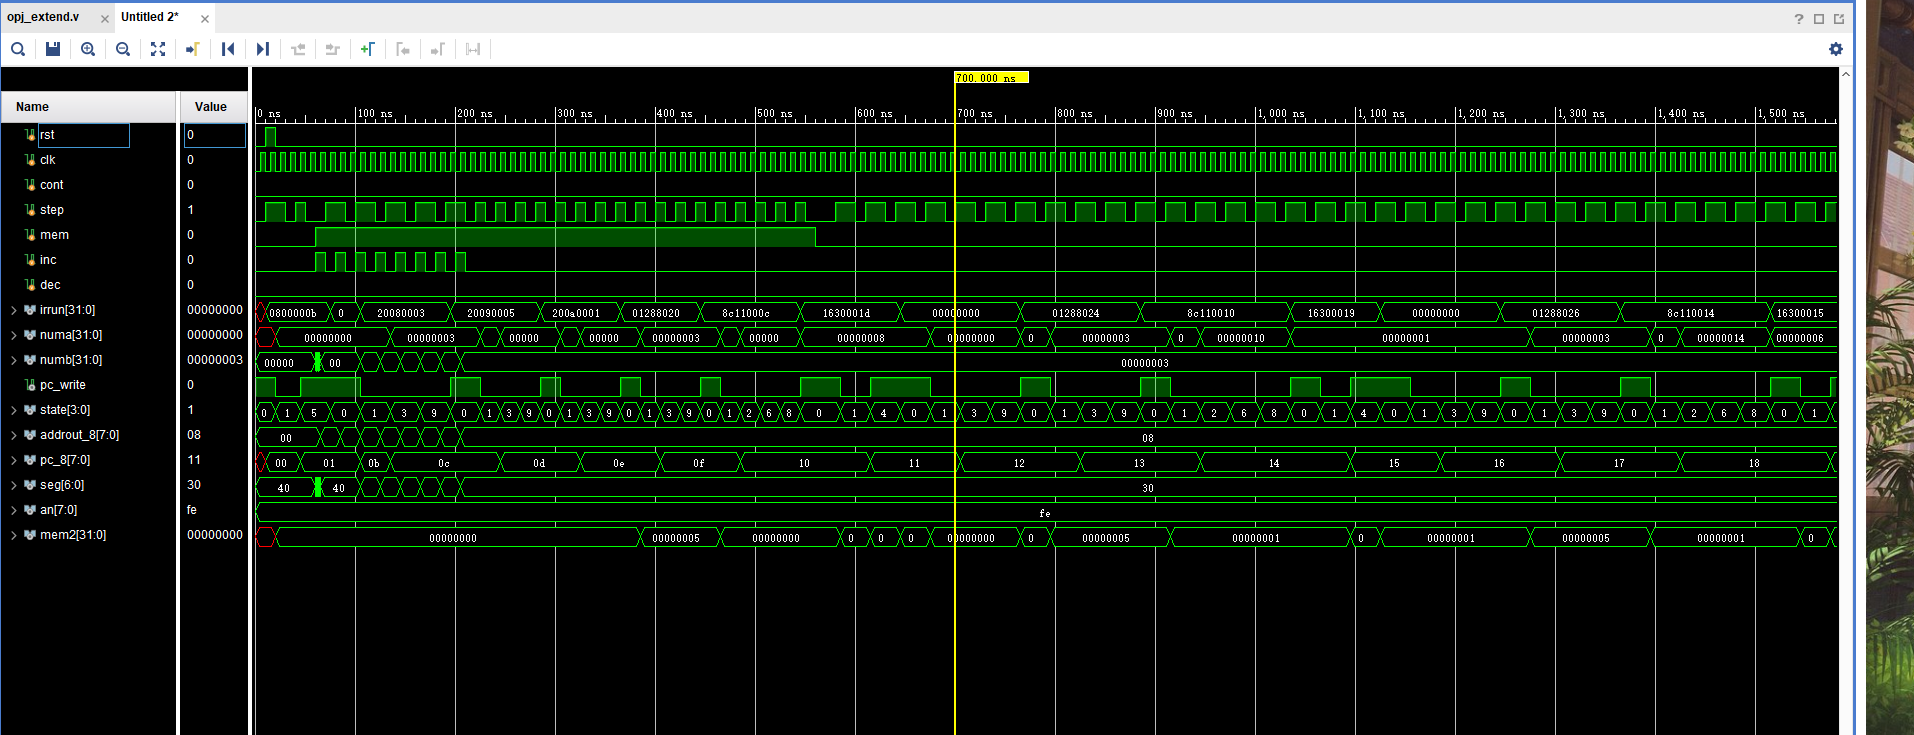
\includegraphics[width=1\linewidth]{pics/sim1}
	\caption{simulation1}
	\label{fig:sim1}
\end{figure}
\begin{figure}[H]
\centering
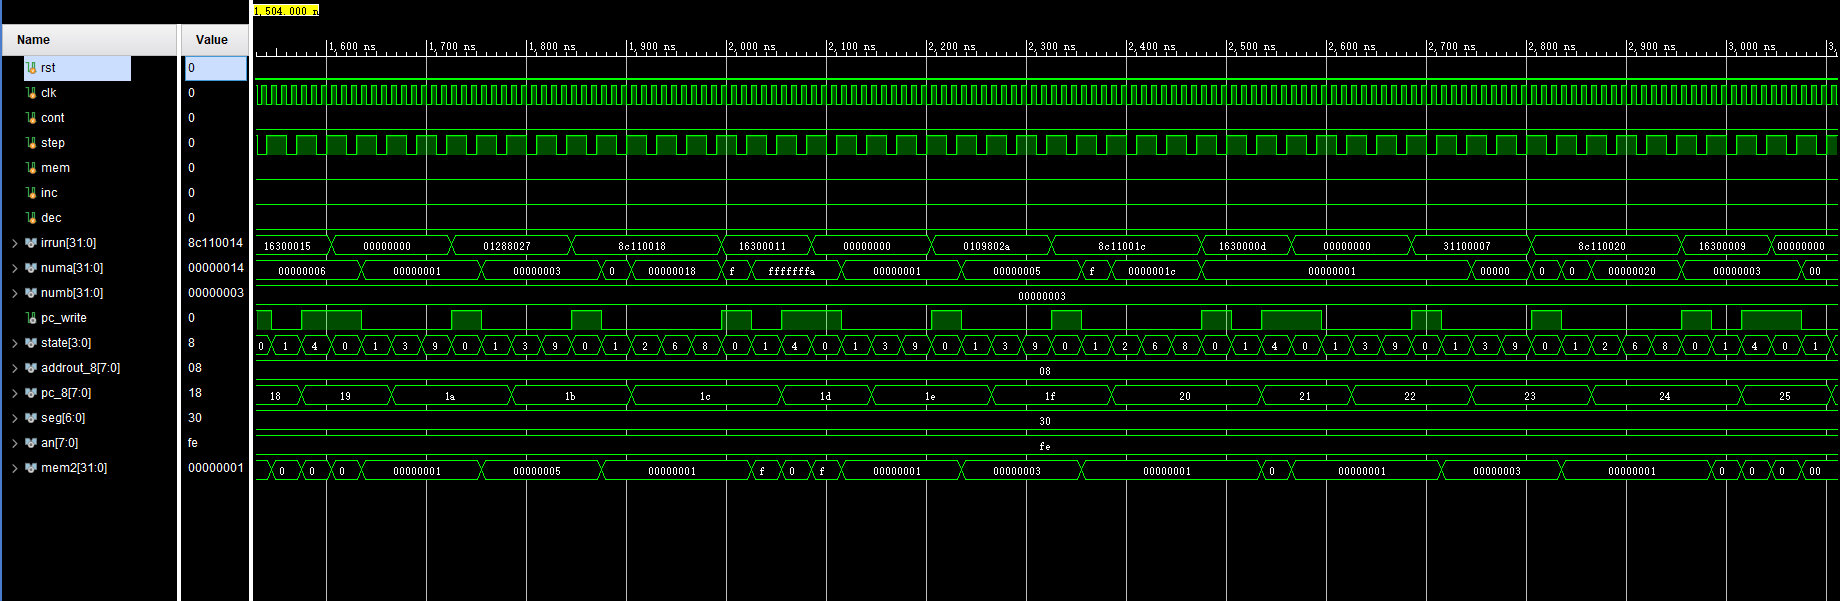
\includegraphics[width=1\linewidth]{pics/sim2}
\caption{simulation2}
\label{fig:sim2}
\end{figure}
\begin{figure}[H]
\centering
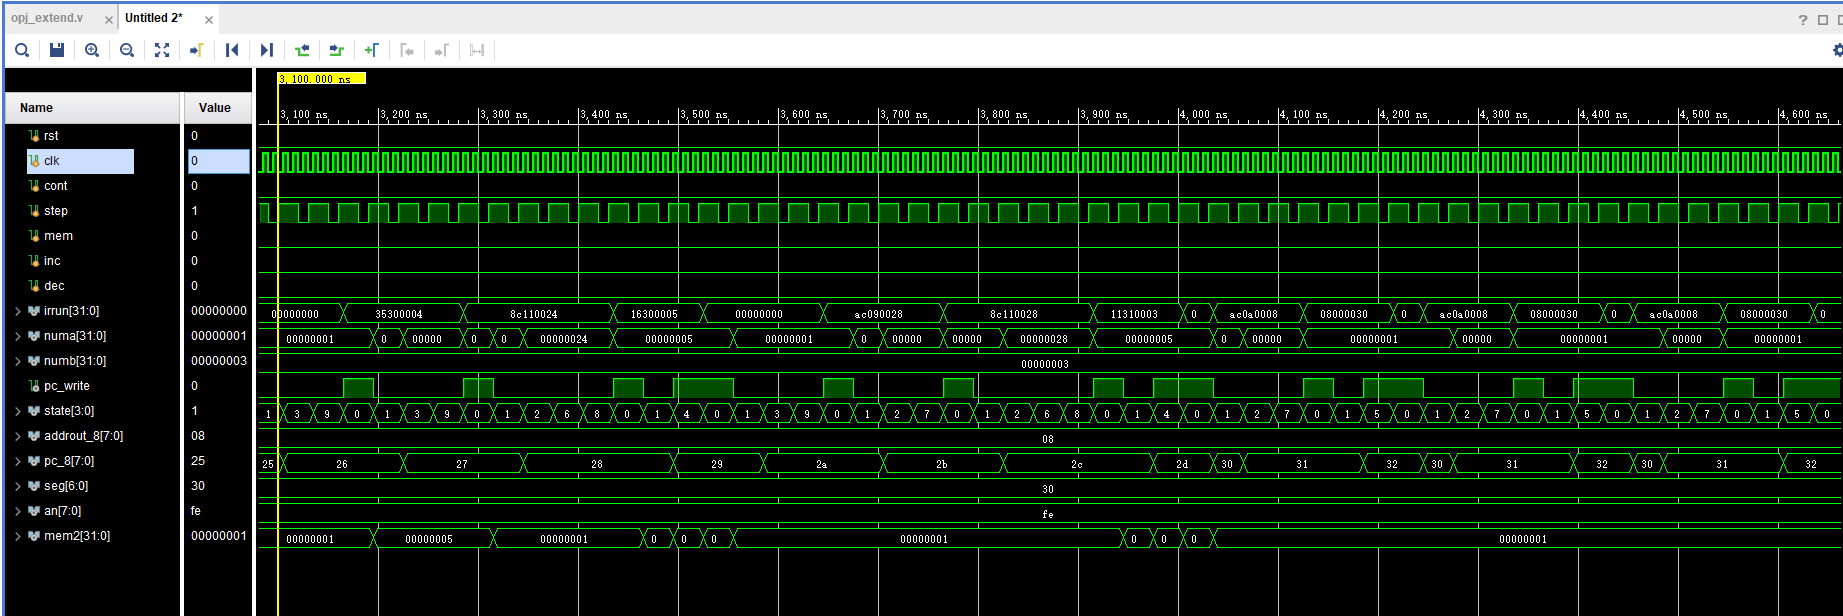
\includegraphics[width=1\linewidth]{pics/sim3}
\caption{simulation3}
\label{fig:sim3}
\end{figure}
拼接起来看图,最终确实进入了那个关于success的死循环之中。

\section{性能评测截图}
\begin{figure}[H]
	\centering
	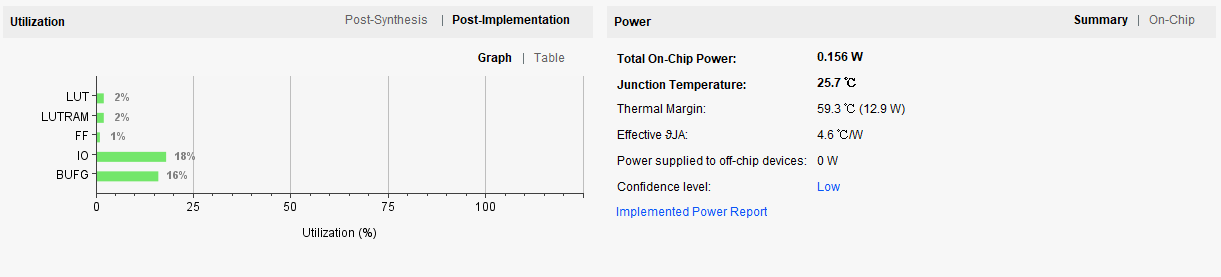
\includegraphics[width=1\linewidth]{pics/per1}
	\caption{performance1}
	\label{fig:per1}
\end{figure}
\begin{figure}[H]
	\centering
	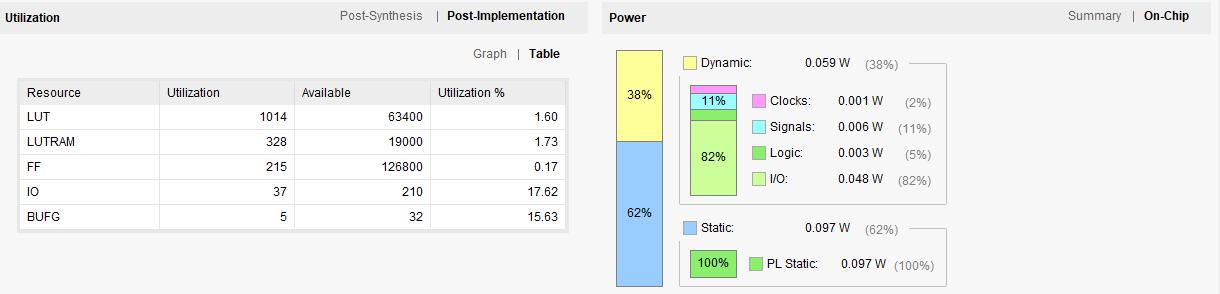
\includegraphics[width=1\linewidth]{pics/per2}
	\caption{performance2}
	\label{fig:per2}
\end{figure}



\section{实验代码}
\subsection {烧写板版本代码}
\lstinputlisting[style={verilog-style},caption={alu.v}]{/home/chivier_humber/Documents/Study/COD_LAB/LAB5/Multicycle/Multicycle.srcs/sources_1/new/alu.v}

\lstinputlisting[style={verilog-style},caption={alu\_ctrl.v}]{/home/chivier_humber/Documents/Study/COD_LAB/LAB5/Multicycle/Multicycle.srcs/sources_1/new/alu_ctrl.v}

\lstinputlisting[style={verilog-style},caption={bcd27.v}]{/home/chivier_humber/Documents/Study/COD_LAB/LAB5/Multicycle/Multicycle.srcs/sources_1/new/bcd27.v}

\lstinputlisting[style={verilog-style},caption={control.v}]{/home/chivier_humber/Documents/Study/COD_LAB/LAB5/Multicycle/Multicycle.srcs/sources_1/new/control.v}

\lstinputlisting[style={verilog-style},caption={cpu.v}]{/home/chivier_humber/Documents/Study/COD_LAB/LAB5/Multicycle/Multicycle.srcs/sources_1/new/cpu.v}

\lstinputlisting[style={verilog-style},caption={ddu.v}]{/home/chivier_humber/Documents/Study/COD_LAB/LAB5/Multicycle/Multicycle.srcs/sources_1/new/ddu.v}

\lstinputlisting[style={verilog-style},caption={define.v}]{/home/chivier_humber/Documents/Study/COD_LAB/LAB5/Multicycle/Multicycle.srcs/sources_1/new/define.v}

\lstinputlisting[style={verilog-style},caption={extend.v}]{/home/chivier_humber/Documents/Study/COD_LAB/LAB5/Multicycle/Multicycle.srcs/sources_1/new/extend.v}

\lstinputlisting[style={verilog-style},caption={ins\_split.v}]{/home/chivier_humber/Documents/Study/COD_LAB/LAB5/Multicycle/Multicycle.srcs/sources_1/new/ins_split.v}

\lstinputlisting[style={verilog-style},caption={mdr.v}]{/home/chivier_humber/Documents/Study/COD_LAB/LAB5/Multicycle/Multicycle.srcs/sources_1/new/mdr.v}

\lstinputlisting[style={verilog-style},caption={mem.v}]{/home/chivier_humber/Documents/Study/COD_LAB/LAB5/Multicycle/Multicycle.srcs/sources_1/new/mem.v}

\lstinputlisting[style={verilog-style},caption={mux2.v}]{/home/chivier_humber/Documents/Study/COD_LAB/LAB5/Multicycle/Multicycle.srcs/sources_1/new/mux2.v}

\lstinputlisting[style={verilog-style},caption={opj\_extend.v}]{/home/chivier_humber/Documents/Study/COD_LAB/LAB5/Multicycle/Multicycle.srcs/sources_1/new/opj_extend.v}

\lstinputlisting[style={verilog-style},caption={pc\_reg.v}]{/home/chivier_humber/Documents/Study/COD_LAB/LAB5/Multicycle/Multicycle.srcs/sources_1/new/pc_reg.v}

\lstinputlisting[style={verilog-style},caption={regfile.v}]{/home/chivier_humber/Documents/Study/COD_LAB/LAB5/Multicycle/Multicycle.srcs/sources_1/new/regfile.v}

\lstinputlisting[style={verilog-style},caption={segout.v}]{/home/chivier_humber/Documents/Study/COD_LAB/LAB5/Multicycle/Multicycle.srcs/sources_1/new/segout.v}

\lstinputlisting[style={verilog-style},caption={constraints.xdc}]{/home/chivier_humber/Documents/Study/COD_LAB/LAB5/Multicycle/Multicycle.srcs/constrs_1/new/constraints.xdc}

\subsection{模拟版本代码}
模拟版本代码中cpu和ddu以及一些模块有所不同,添加了更多的wire output取显示更多的调试信息。\\
下面仅贴出不同部分的代码,其余相同部分不再重复复制。

\lstinputlisting[style={verilog-style},caption={cpu.v}]{/home/chivier_humber/Documents/Study/COD_LAB/LAB5/Multicyclesim/Multicycle.srcs/sources_1/new/cpu.v}

\lstinputlisting[style={verilog-style},caption={ddu.v}]{/home/chivier_humber/Documents/Study/COD_LAB/LAB5/Multicyclesim/Multicycle.srcs/sources_1/new/ddu.v}

\lstinputlisting[style={verilog-style},caption={regfile.v}]{/home/chivier_humber/Documents/Study/COD_LAB/LAB5/Multicyclesim/Multicycle.srcs/sources_1/new/regfile.v}

\lstinputlisting[style={verilog-style},caption={control.v}]{/home/chivier_humber/Documents/Study/COD_LAB/LAB5/Multicyclesim/Multicycle.srcs/sources_1/new/control.v}

\lstinputlisting[style={verilog-style},caption={cpu\_sim1.v}]{/home/chivier_humber/Documents/Study/COD_LAB/LAB5/Multicyclesim/Multicycle.srcs/sim_1/new/cpu_sim1.v}

\section {总结}
本次实验相当于一次比较综合的复习,复习了我们学习COD至多周期的各种知识。本次实验对于我来说最大的困难就是如何将程序正确的烧写到板子上。事实上,我只用了3天就完成了正确的模拟和仿真,但是到最终完成花费了整整3周的时间。具体原因在于对于时序逻辑和组合逻辑的写法规范性。

举个例子,再我extend的模块中,本来应该用wire就可以完成的任务,就不必多加一个reg进行中介保存,虽然理论上有着一样的效果,但是实际上,这样的代码过多会倒置无意义的锁存现象出现,从而出现各种诡异的bug出现。此外另一个困扰我整整一周的实验bug是板载时钟周期过短,无法再一个时钟周期内完成应该执行完成的任务,出现了神奇的bug。

最终,实验也再截止日期前完成,总体来说还算顺利。

\section{意见和建议}
本次实验个人感觉,难度并不是很大,但是再我们烧写板子的时候,比较考研问题分析解决能力和动手能力。个人建议,之后实验助教要求检查的只有我们的仿真模拟,至于烧录可以考虑作为附加分处理。

此外,我决定我们之后可以增加一次关于流水实现的实验,也是只要求模拟,不要求仿真。考虑流水的复杂性和代码量,个人认为,设计流水CPU再多周期之后,并且要求同学们合作完成。这样可以达到更好的效果。

最后表示,老师还是最好不要删除单周期的实验,第一在于……通知太晚,我都写完了才说取消实验。第二在于,单周期作为复习也是很有必要的。而且,如果单周期的实验吐过顺利完成,之后的多周期会少很多问题,例如办在诗中的处理和锁存器等等。
\end{document}
